\section{Patching, Compiling, Installing, and Booting Your Custom Linux Kernel}
The following instructions were adapted from the NDT cookbook, found \href{www.internet2.edu/pubs/ndt-cookbook.pdf‎}{here}.\footnote{www.internet2.edu/pubs/ndt-cookbook.pdf‎}

\subsection{Getting and Unpacking Resources}
Getting and unpacking the linux kernel: 
\begin{snugshade}\begin{verbatim}
$ cd /usr/src
$ sudo mkdir tars
$ cd tars
$ sudo wget https://www.kernel.org/pub/linux/kernel/v2.6/linux-2.6.32.tar.gz
$ sudo tar -xvf ./linux-2.6.32.tar.gz
$ sudo mv ./linux-2.6.32 /usr/src/kernels/linux-2.6.32
\end{verbatim}\end{snugshade}\noindent
Getting and unpacking the web100 patch
\begin{snugshade}\begin{verbatim}
$ cd /usr/src/tars
$ sudo wget http://www.web100.org/download/kernel/2.5.27/web100-2.5.27-201001301335.tar.gz
$ sudo tar -xvf ./web100-2.5.27-201001301335.tar.gz
$ sudo mkdir /usr/src/kernel_patches
$ sudo mv ./web100 /usr/src/kernel_patches/web100
\end{verbatim}\end{snugshade}\noindent

\hrule


\subsection{Patching Kernel}
To apply the web100 patch to the linux kernel, issue the commands below:
\begin{snugshade}\begin{verbatim}
$ cd /usr/src/kernels/linux-2.6.32
$ sudo patch -p1 < /usr/src/kernel_patches/web100/web100-2.6.32-2.5.27-201001301335.patch 
\end{verbatim}\end{snugshade}\noindent

\hrule

\subsection{Compiling and Configuring Kernel}
To compile the kernel, issue the following commands:
\begin{snugshade}\begin{verbatim}
$ cd /usr/src/kernels/linux-2.6.32
$ make clean
$ make mrproper
\end{verbatim}\end{snugshade}\noindent
Copy the current kernel's boot config to our new kernel:
\begin{snugshade}\begin{verbatim}
$ sudo cp /boot/config-2.6.32-358.el6.x86_64 ./.config
\end{verbatim}\end{snugshade}\noindent
Configure the kernel: 
\begin{snugshade}\begin{verbatim}
$ sudo make menuconfig
\end{verbatim}\end{snugshade}\noindent
The configuration screen should load eventually. Follow the guide on the next few pages through the menuconfig GUI.
\newpage

\begin{enumerate}
\item{Navigate to \textit{Networking Support} and hit enter.}
\begin{figure}[H]
\centering
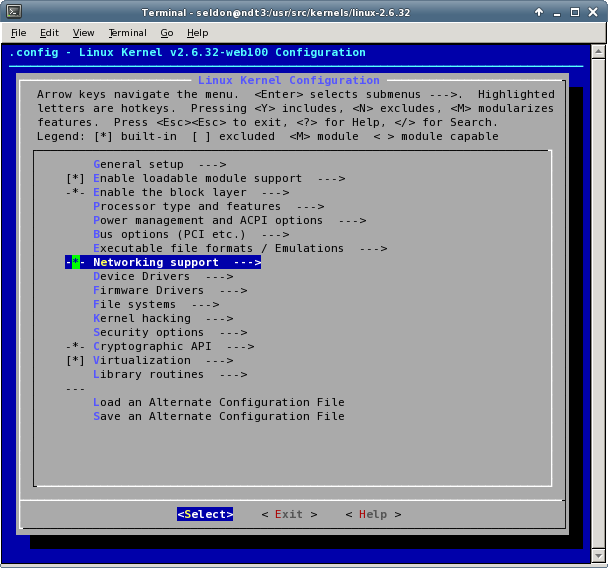
\includegraphics[width=.55\textwidth]{img/menuconfig_01.png}
\end{figure}

\item{Navigate to \textit{Networking Options} and hit enter.}
\begin{figure}[H]
\centering
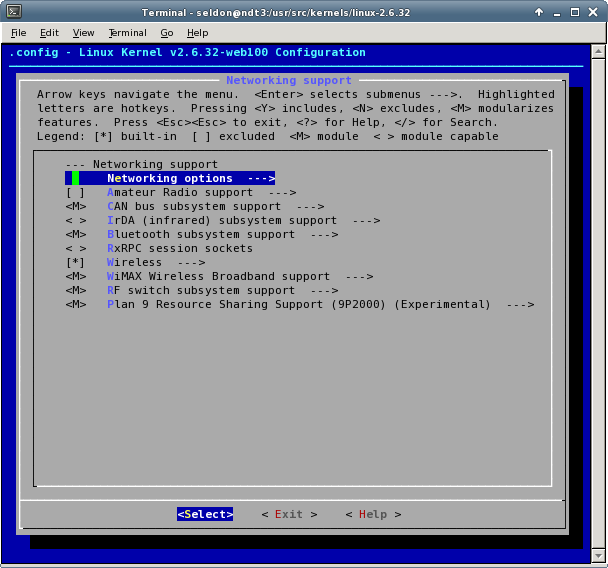
\includegraphics[width=.55\textwidth]{img/menuconfig_02.png}
\end{figure}

\item{Navigate to \textit{IP Web100 Networking Enhancements} and press y followed by enter.}
\begin{figure}[H]
\centering
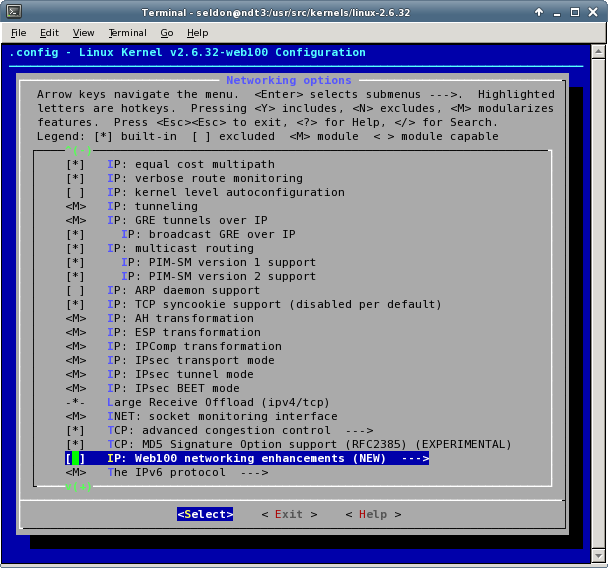
\includegraphics[width=.55\textwidth]{img/menuconfig_03.png}
\end{figure}

\item{Press y over \textit{Web100 Extended TCP/IP Statistics}.}
\item{Ensure that the newly spawned \textit{Web100: Default File Permissions} and \textit{Default GID} match with the image below.}
\item{Press y over \textit{Web100: Net100 extensions} and \textit{Web100: Netlink Event Notification Service}.}

\begin{figure}[H]
\centering
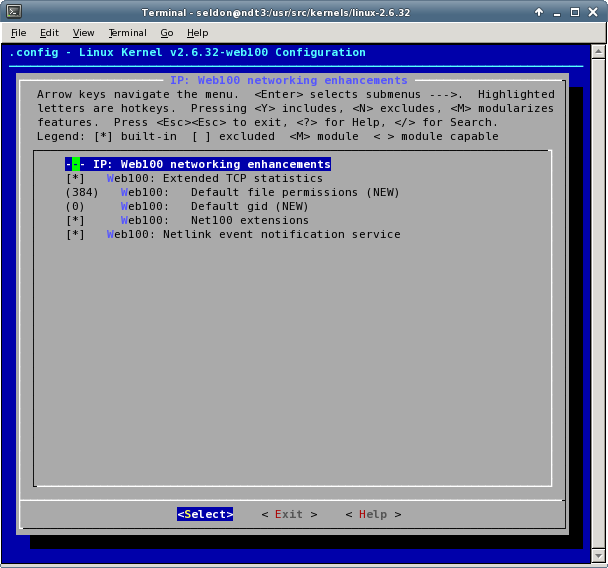
\includegraphics[width=.55\textwidth]{img/menuconfig_05.png}
\end{figure}

\item{Press escape twice.}
\item{Select yes and press enter when prompted to save your config,}

\begin{figure}[H]
\centering
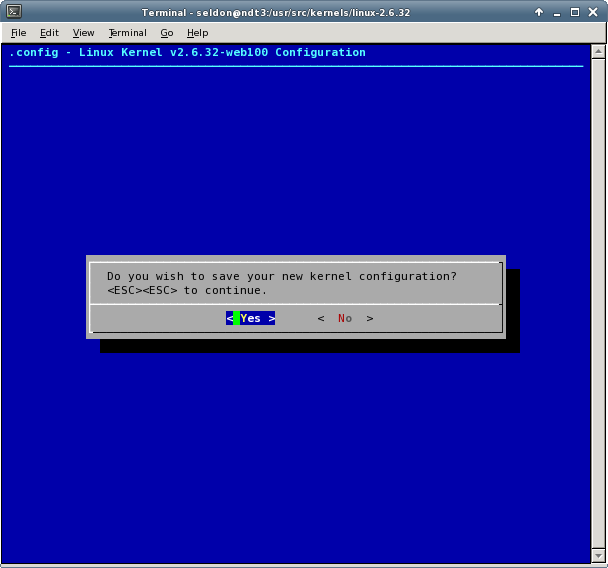
\includegraphics[width=.55\textwidth]{img/menuconfig_06.png}
\end{figure}
\end{enumerate}

\hrule

\subsection{Making RPM file}
To begin making the RPM file, ensure first that you have made the RPMBUILD environment as described in this tutorial, and issue the following commands (this will take about 30 minutes):
\begin{snugshade}\begin{verbatim}
$ cd /usr/src/kernels/linux-2.6.32
$ sudo make rpm 
\end{verbatim}\end{snugshade}\noindent
Now you must find where your RPM file was placed. If all went well, it should be in your RPMBUILD directory structure. However, it may end up in /root/rpmbuild. If this is the case, do the following:
\begin{snugshade}\begin{verbatim}
$ su
# cp -ar /root/rpmbuild /home/seldon/
# chown -R seldon /home/seldon/rpmbuild
# exit
$ chmod 777 ~/rpmbuild
\end{verbatim}\end{snugshade}\noindent 

\hrule

\subsection{Installing Your RPM File}

once your rpm is in your home directory:
\begin{snugshade}\begin{verbatim}
$ cd /home/seldon/rpmbuild/RPMS/x86_64
$ sudo rpm -ivh kernel-2.6.32web100-1.x86_64.rpm
\end{verbatim}\end{snugshade}\noindent

\subsection{Preparing to Boot}
Type the following into the terminal: 
\begin{snugshade}\begin{verbatim}
$ sudo mkinitrd /boot/initrd-2.6.32web100.img 2.6.32-web100
\end{verbatim}\end{snugshade}\noindent

\hrule

\subsection{Configuring GRUB}

To begin configuring grub, type the following into the terminal:
\begin{snugshade}\begin{verbatim}
$ sudo gedit /etc/grub.conf
\end{verbatim}\end{snugshade}\noindent
My grub.conf looked like this: 
\begin{snugshade}\begin{lstlisting}
# grub.conf generated by anaconda
#
# Note that you do not have to rerun grub after making changes to this file
# NOTICE:  You have a /boot partition.  This means that
#          all kernel and initrd paths are relative to /boot/, eg.
#          root (hd0,0)
#          kernel /vmlinuz-version ro root=/dev/sda3
#          initrd /initrd-[generic-]version.img
#boot=/dev/sda
default=0
timeout=5
splashimage=(hd0,0)/grub/splash.xpm.gz
hiddenmenu
title CentOS (2.6.32-358.18.1.el6.x86_64)
       root (hd0,0)
       kernel /vmlinuz-2.6.32-358.18.1.el6.x86_64 ro root=UUID=e500f799-a5d4-485d-ba19-9a6537a94dc1 nomodeset rd_NO_LUKS  KEYBOARDTYPE=pc KEYTABLE=us LANG=en_US.UTF-8 rd_NO_MD SYSFONT=latarcyrheb-sun16 crashkernel=128M rd_NO_LVM rd_NO_DM rhgb quiet
       initrd /initramfs-2.6.32-358.18.1.el6.x86_64.img
title CentOS (2.6.32-358.el6.x86_64)
       root (hd0,0)
       kernel /vmlinuz-2.6.32-358.el6.x86_64 ro root=UUID=e500f799-a5d4-485d-ba19-9a6537a94dc1 nomodeset rd_NO_LUKS  KEYBOARDTYPE=pc KEYTABLE=us LANG=en_US.UTF-8 rd_NO_MD SYSFONT=latarcyrheb-sun16 crashkernel=128M rd_NO_LVM rd_NO_DM rhgb quiet
	initrd /initramfs-2.6.32-358.el6.x86_64.img
\end{lstlisting}\end{snugshade}\noindent
I changed it so that it looks like this: 
\begin{snugshade}\begin{lstlisting}
# grub.conf generated by anaconda
#
# Note that you do not have to rerun grub after making changes to this file
# NOTICE:  You have a /boot partition.  This means that
#          all kernel and initrd paths are relative to /boot/, eg.
#          root (hd0,0)
#          kernel /vmlinuz-version ro root=/dev/sda3
#          initrd /initrd-[generic-]version.img
#boot=/dev/sda
default=0
timeout=5
splashimage=(hd0,0)/grub/splash.xpm.gz
#hiddenmenu
title CentOS-Web100 (2.6.32-358)
       root (hd0,0)
       kernel /vmlinuz-2.6.32-web100 root=UUID=e500f799-a5d4-485d-ba19-9a6537a94dc1 nomodeset rd_NO_LUKS  KEYBOARDTYPE=pc KEYTABLE=us LANG=en_US.UTF-8 rd_NO_MD SYSFONT=latarcyrheb-sun16 crashkernel=128M rd_NO_LVM rd_NO_DM rhgb quiet
       initrd /initrd-2.6.32web100.img
title CentOS (2.6.32-358.18.1.el6.x86_64)
       root (hd0,0)
       kernel /vmlinuz-2.6.32-358.18.1.el6.x86_64 ro root=UUID=e500f799-a5d4-485d-ba19-9a6537a94dc1 nomodeset rd_NO_LUKS  KEYBOARDTYPE=pc KEYTABLE=us LANG=en_US.UTF-8 rd_NO_MD SYSFONT=latarcyrheb-sun16 crashkernel=128M rd_NO_LVM rd_NO_DM rhgb quiet
       initrd /initramfs-2.6.32-358.18.1.el6.x86_64.img
title CentOS (2.6.32-358.el6.x86_64)
       root (hd0,0)
       kernel /vmlinuz-2.6.32-358.el6.x86_64 ro root=UUID=e500f799-a5d4-485d-ba19-9a6537a94dc1 nomodeset rd_NO_LUKS  KEYBOARDTYPE=pc KEYTABLE=us LANG=en_US.UTF-8 rd_NO_MD SYSFONT=latarcyrheb-sun16 crashkernel=128M rd_NO_LVM rd_NO_DM rhgb quiet
	initrd /initramfs-2.6.32-358.el6.x86_64.img
\end{lstlisting}\end{snugshade}\noindent
I did this in the following steps: 
\begin{enumerate}
\item{Uncomment the \textit{hiddenmenu} line to force grub to load.}
\item{Made a new kernel entry before all of the other entries: }
\begin{itemize}
\item{CentOS-Web100 (2.6.32-358)}
\item{For the kernel part of the entry, I specified the web100 kernel, but then the rest of the line I had to borrow from the entry below, which is the kernel that you should be launched in now.}
\end{itemize}
\end{enumerate}
Now save and quit gedit, and reboot your system:
\begin{snugshade}\begin{verbatim}
$ sudo reboot
\end{verbatim}\end{snugshade}\noindent
GRUB should load, and you should select \textit{CentOS-Web100 (2.6.32-358)} and wait for it to load. Once it loads, login to seldon.
































\newpage
